\chapter{Required Properties of E2E Systems\ifdraft{ (Dan) (100\%)}{}}
\label{chapter:required_properties}

In August 2010, the U.S. Election Assistance Commission issued a set
of testing requirements for overseas and military remote electronic
voting system pilot projects~\cite{eac-uocava2010}. However, the EAC
requirements have some serious shortcomings. Many of the requirements
are arbitrary, inappropriate, or invalid: some set maximum system
error rates using specific numbers without justifying the numbers;
some set unrealistic limits on the accuracy of computer hardware; and
some prohibit developers from programming in ways that are widely used
when implementing highly reliable software systems.

% This is the original text; I'm keeping it here for reference, but
% significantly shortening it. -dmz
%
% The general
% categories of requirements specified by the EAC included functional
% requirements, such as the need for the system to produce paper records
% of voter choices and generate human-readable ballot images;
% requirements on software development, such as allowable programming
% languages and coding conventions; usability, accessibility and privacy
% requirements, such as that a voter's ballot choices must remain
% private and that provisions must be made to support voters with
% disabilities; security requirements, including logging requirements,
% requirements on communications security within the system, and
% requirements on physical security and penetration resistance; quality
% assurance requirements describing the testing that must be done on the
% systems; and requirements about configuration management mechanisms,
% technical information, and documentation to be provided by system
% vendors.

% The EAC requirements have some serious shortcomings, one of which is
% that several of the requirements seem arbitrary. For example, they
% specify (in Section 2.1 of the requirements document) that the voting
% system shall achieve a target error rate of no more than one in
% 10,000,000 ballot positions, with a maximum acceptable error rate in
% the test process of one in 500,000 ballot positions, without any
% justification for those numbers. They further specify (in Sections
% 2.1.1.1--2) that ``memory hardware, such as semiconductor devices and
% magnetic storage media, shall be accurate'' and that ``the design of
% equipment in all voting systems shall provide for protection against
% mechanical, thermal, and electromagnetic stresses that impact voting
% system accuracy'' without any guidance on how to evaluate such
% accuracy or protective ability.

% In addition to these shortcomings, some of the EAC requirements are
% inappropriate or invalid. The most obvious example of this is the set
% of requirements that mandate specific ``structured programming''
% characteristics of software implementation languages (Sections 4.1 and
% 4.4), which seem to eliminate functional programming languages such as
% Haskell and Erlang---widely used in implementing high-assurance
% systems---from consideration entirely.

If these issues were addressed, the EAC requirements could serve as a
solid set of requirements for remote electronic voting
systems. However, they are not strong enough to guarantee end-to-end
verifiability, which is essential when considering Internet voting
systems for use in real elections.  

A set of E2E-VIV requirements, which significantly overlaps with the
EAC requirements, can be broadly divided into two groups:
\emph{technical requirements} and \emph{non-functional
  requirements}. Technical requirements are those that can be directly
addressed by the design and implementation of the system, such as
authentication requirements for voters and election
officials. Non-functional requirements are those that are imposed on
the system by external entities or where the system depends on
external behaviors outside its control, such as specific election
certification guidelines and operational procedures. The technical and
non-functional requirement groups can be further divided into several
categories, and \autoref{fig:e2eviv_requirements_hierarchy} gives a
high-level overview of these.

The following is a high-level description of the E2E-VIV requirement
categories and many of the requirements; the full set of E2E-VIV
requirements expressed in the Business Object Notation is available as
a separate document~\cite{E2EVIVBON}.

%=====================================================================
\section{Technical Requirements}
There are ten categories of technical requirements for E2E-VIV
systems: functional, accessibility, usability, security,
authentication, auditing, system operational, reliability,
interoperability, and certification. 

\clearpage\break

%~~~~~~~~~~~~~~~~~~~~~~~~~~~~~~~~~~~~~~~~~~~~~~~~~~~~~~~~~~~~~~~~~~~~~
\subsection{Functional} 
\label{sec:functional}

\begin{wrapfigure}[45]{r}{3.25in}
\begin{center}
\vspace*{-5ex}
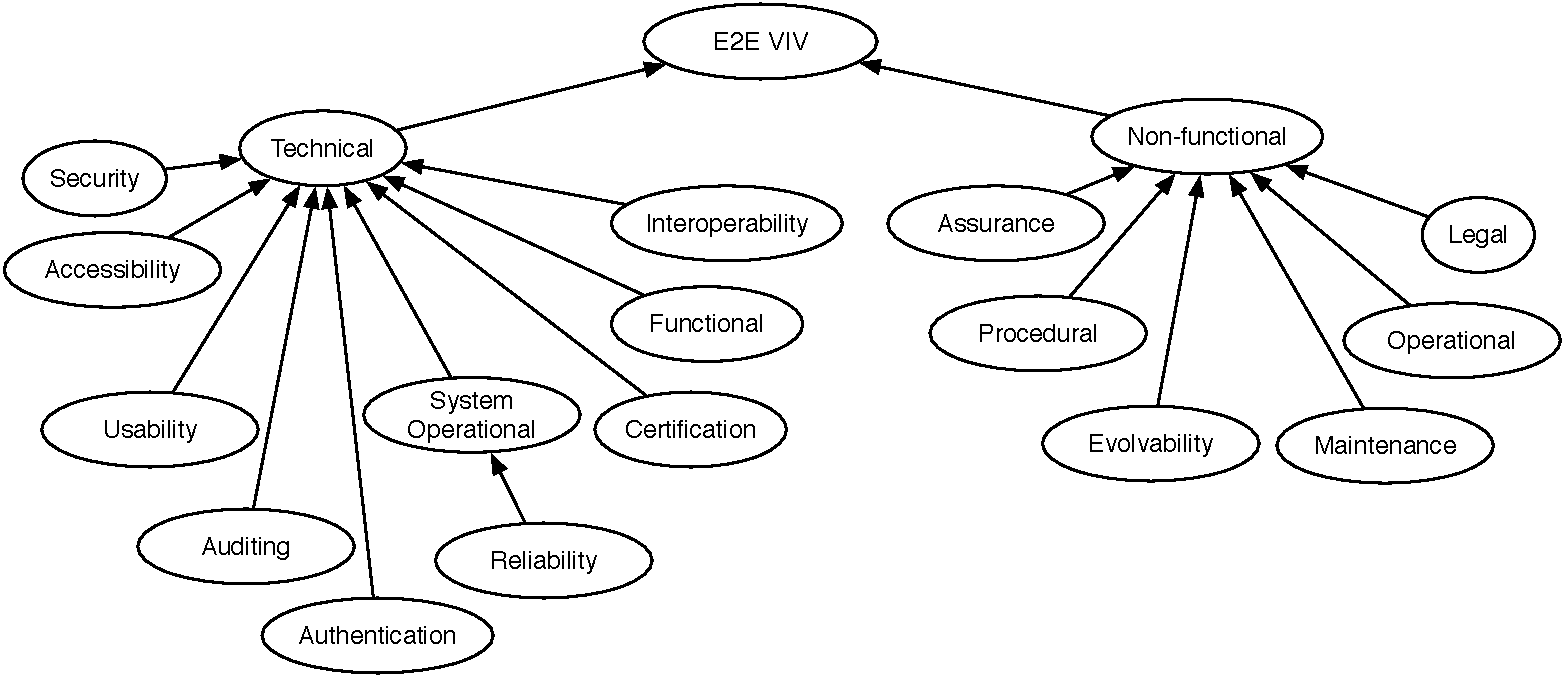
\includegraphics[width=3in]{required_properties_resources/hierarchy}
\end{center}
\caption{Requirements hierarchy for E2E-VIV systems.}
\label{fig:e2eviv_requirements_hierarchy}
\end{wrapfigure}

The functional requirements of an E2E-VIV system deal primarily with
the casting and recording of ballots and associated voter records. One
such requirement is that recorded ballots and voters listed as having
voted must correspond with each other; a ballot cannot be recorded
without a voter casting it, and a voter cannot be listed as having
voted without casting a ballot. If the system tells a voter that her
ballot has been successfully cast, the system must correctly retain
the record that she has voted. The system must keep a voter's cast
ballot information even if servers fail.

Another functional requirement is \emph{receipt freedom}: it must be
impossible for a voter to prove to anybody any information regarding
how she voted, beyond what someone can mathematically deduced from the
final distribution of votes. If a referendum passes with 100\% of the
vote, for example, there is no way to hide the fact that every voter
approved of the referendum. If the result is mixed, it must be
impossible for any individual voter to prove how she voted.  This must
be true even when the voter can create digital evidence of her actions
by, for example, video recording the ballot casting process or
photographing a completed ballot. 

No usable E2E-VIV protocol in existing scientific literature has
receipt freedom when the voting computer is untrusted. Since the
process of casting any individual ballot can be recorded, a protocol
with receipt freedom must allow the voter to vote multiple times but
only count the last ballot a voter casts. However, it must also ensure
that an observer watching any recorded ballot casting process can
independently verify that the ballot was cast. This must be ensured
even when the voting computer is not trusted to follow protocol, and
in a manner that is easy to use and accessible. This represents a
significant research challenge for E2E-VIV protocol designers.

In some elections, voters are allowed to cast multiple ballots with
only the last cast ballot counting toward the final election tally. In
others, voters are prohibited from casting multiple ballots. The
system must accommodate both of these election formats.

Maintaining voter anonymity is critical. It must be impossible after
the election to reconstruct a link between a cast ballot and any
identifying information about the voter who cast it. However, in
systems that support the casting of multiple ballots, it is important
to maintain links between voters and their ballots \emph{during} the
election to ensure that later ballots replace earlier ballots. To
balance these concerns, any link between a ballot and the voter who
cast it must be irrevocably broken once it is determined that the
ballot will be counted toward the final tally.

% I'm commenting this one out because it doesn't really go with the
% others, but of course it will still be in the appendix -dmz
%
% Finally, because the voter should be able to focus on the voting
% process without undue distractions or external influences, the voting
% system must not display or permit the display of any advertising or
% commercial logos during a voting session; the exception to this rule
% is that an election jurisdiction may display its own logo to the voter
% during the voting process. Along the same lines, the voting system
% must not display any links to other Internet sites outside of the
% voting system, except to provide help with the actual mechanics of
% voting.

%~~~~~~~~~~~~~~~~~~~~~~~~~~~~~~~~~~~~~~~~~~~~~~~~~~~~~~~~~~~~~~~~~~~~~
\withicon{usability}{\subsection{Usability}}

The usability of an E2E-VIV system is critical to its successful
adoption and use. Since user experience is so important, many of the
requirements of the system have some relation to usability even though
they may be categorized under other headings. There are, however, two
requirements that are exclusively related to the usability of the
system with respect to vote casting and a general usability
requirement that applies to the system as a whole.

If a voter receives a final vote confirmation from the system, such as
``Thank you for voting!'', the ballot casting process must be complete
and the system must have recorded the vote. This allows voters to be
certain that their ballots have been recorded and will be counted.

If a voter is uncertain whether or not the system recorded her
ballot---for example, she clicked a ``submit'' button but never got a
response from the system---she must be able to vote again.

Researchers must perform usability testing on any E2E-VIV system
before it is deployed. The reports of the usability testing must be
made public, and the system must achieve satisfactory test results
before election officials use it in a real election.

%~~~~~~~~~~~~~~~~~~~~~~~~~~~~~~~~~~~~~~~~~~~~~~~~~~~~~~~~~~~~~~~~~~~~~
\withicon{accessibility}{\subsection{Accessibility}}

Accessibility---the property of being usable by and useful to voters
with disabilities---is one of the main goals of an E2E-VIV system. It
is closely related to usability, but there are several requirements
associated specifically with accessibility that go beyond typical
usability requirements.

Users must be involved in the design of the system to identify
accessibility problems at each stage of the development
process. Developers must consider the system's compatibility with
existing technologies designed to help individuals with disabilities.
The system should be developed in a way that allows people to use
accessible devices such as switches, eye trackers and screen readers
in addition to keyboards, mice and touchscreens. The system should
present voting options that are optimized for voters' needs by using
alternative display fonts, audio representations, braille
representations, and other representations as appropriate.

Developers must take all possible measures to ensure that as many
voters as possible can use the system. Election officials must provide
access to alternative methods of voting for those voters who cannot
use the system.

Researchers must perform accessibility testing in addition to
mandatory usability testing. The reports of the accessibility testing
must be made public, and the system must achieve satisfactory test
results before election officials use it in a real election.

\clearpage\break

%~~~~~~~~~~~~~~~~~~~~~~~~~~~~~~~~~~~~~~~~~~~~~~~~~~~~~~~~~~~~~~~~~~~~~
\withicon{security_and_authentication}{\subsection{Security and
Authentication}}

Security and authentication are closely related. Together, they
represent the broadest set of technical requirements. These include
requirements on the E2E-VIV system itself, such as data storage and
communications, and requirements on the voting and counting processes
that the system enables, including voter authorization, voter privacy,
vote integrity, and tally accuracy.

Developers must ensure data integrity throughout the system.  No data
can be permanently lost if the system breaks down or experiences a
fault. The system must maintain the integrity of the voters' register,
lists of candidates, ballot information, cast ballots, and other
critical information. It must authenticate the original source(s) of
all information and keep track of where the information came from. All
data communications within the system must have associated integrity
checks.

System equipment under the control of election officials must be
protected against influences that could modify election results. The
integrity of the election results must not depend, in any way, upon
the security of system equipment that election officials do not
control. The system must perform regular ``health checks'' to ensure
that it is maintaining data integrity, all its components are
operating in accordance with their specifications, and all system
services are available.

Accurate timing information is critical to security, both to provide
evidence of compliance with applicable regulations and to detect
attacks on and potential breaches of the system. The system must
therefore maintain reliable synchronized time sources, with sufficient
accuracy to maintain timing data for audit information, election
observation data, and time limits for various aspects of the election
process. Using the timing information stored by the system, it must be
possible to determine whether nominations (and, if required, the
candidate's or election officials' acceptance), voter registration,
and vote casting occurred within the time limits for those actions.

Authentication and authorization are also important aspects of
security. The system must ensure that each individual can be
identified uniquely, so that there is no possibility of mistaking one
individual for another. The system must also maintain the privacy of
individuals, by ensuring that all personally identifiable data is kept
confidential as far as legal requirements of the electoral
jurisdiction allow. The system must allow access to each of its
services only to authorized users; for example, only election
officials may be allowed to load ballot information into the system.

The means used to gain access to the system must, as far as possible,
protect authentication secrets (passwords, one-time access codes,
biometrics, etc.) so that unauthorized entities cannot acquire
them. People may not use third party authentication mechanisms, such
as existing Facebook, Google and Twitter accounts, to access the
system. 

Any potential breach of any public or commercial database, such as a
credit card database or the Social Security database, must not affect
the security of the voting system's authentication mechanism. An
attacker should not be able to impersonate a voter even if the entire
database used for authentication in the system is
compromised. Individual authentication secrets themselves must be
changeable or revocable at any time, at the individual voter's or
election officials' request. The system should require all individuals
to change their authentication secrets at least at least once in every
election cycle.

The system must allow only eligible voters to cast ballots, and must
ensure that each voter only casts the appropriate number of ballots. A
voter must be able to verify that the system has presented her with an
authentic ballot and, in the case of remote voting, that she has a
secure connection to an official server.

The system must preserve the privacy and integrity of the vote,
end-to-end, to the maximum extent possible. Individual voters may not
waive the privacy of their votes. In the case of remote voting, the
system must preserve vote privacy and integrity even if the voter's
computer contains malicious code (corrupted client software, key
logging software or devices, etc.). Any client software used in remote
voting must not send data to any Internet host except those associated
with the E2E-VIV system or provide any information to third parties
(such as Facebook or Twitter) regarding the act of voting. The system
must destroy any residual information that could be used to discover a
voter's choices after a ballot has been cast. If a voter uses a
computer outside the control of election officials to cast her vote,
she must be provided with instructions for destroying the residual
information on that computer.

The system must accurately count the votes, and the counting process
must be reproducible. The system must also maintain the availability
and integrity of all information used to generate the final tally and
all information regarding the counting process itself for as long as
required. Vote tabulation must be \emph{strongly software
  independent}; it must be possible to detect any compromise of the
election system software that causes a change in the tally, and to
reconstruct a correct tally from some record in the event of such a
compromise.

A deployed E2E-VIV system will likely be an attractive target for
highly capable adversaries who wish to influence election results or
to disrupt election processes. System designers and testers must
assume that an adversary has a budget of US\$10 per voter per election
that they can apply toward any subset of votes or voters of they
choose. This means that designers and testers of an E2E-VIV system for
use in a U.S. presidential election must assume that an adversary has
a budget of approximately US\$1,300,000,000.

Election officials shall have overall responsibility for compliance
with these security requirements, and independent bodies will assess
compliance as appropriate.

%~~~~~~~~~~~~~~~~~~~~~~~~~~~~~~~~~~~~~~~~~~~~~~~~~~~~~~~~~~~~~~~~~~~~~
\withicon{auditing}{\subsection{Auditing}}

The ability to perform comprehensive audits of system activity is one
of the important distinguishing aspects of an E2E-VIV system.
compared to other voting systems. In addition to those security
requirements (such as the tracking of accurate timing information)
that touch on auditing, several system requirements relate
specifically to auditing.

Developers must design and implement audit features as part of the
E2E-VIV system from the beginning; they cannot be added as an
afterthought to an existing system. Developers must implement audit
and monitoring capabilities into all levels of the system, from
low-level communications among individual computers to high-level
interactions with election officials. The system must keep audit logs
of all activity relevant to the conduct and outcome of the
election. These logs must be locked, incapable of being modified by
anyone, once they are written. They must also be as complete as
possible without violating voter privacy.

The audit system must actively report potential issues and threats,
rather than merely serving as a passive repository of system logs. It
must record at least the following events and actions with accurate
timing information: 

\begin{itemize}
\item all voting-related information, including the number of eligible
  voters and votes cast, the number of invalid votes, count and
  recount results, etc.;
\item any detected attacks on the operation of the
  system or its communication infrastructure; and
\item any system failures,
  malfunctions, or other detected threats to proper system
  operation. 
\end{itemize}

The audit system must provide sufficient information to election
observers in real time, and after the election's conclusion, to verify
that the election is carried out in accordance with applicable law.

The audit system must also be able to:

\begin{itemize}
\item cross-check and verify the correct operation of the voting
  system and the accuracy of the election results;
\item detect voter fraud; and 
\item prove that all counted
votes are legitimate and that all ballots have been counted. 
\end{itemize}

In situations where the system cannot verify the legitimacy of all the
votes, it must be able to report how many ballots may be affected.

If a tradeoff must be made between maintaining voter privacy and
identifying the perpetrators of fraud, the system must resolve that
tradeoff in favor of voter privacy.

For voters to trust an E2E-VIV system, its auditability must extend to
its own source code as well as the activities it performs during an
election. Developers must publish the E2E-VIV system software and any
official monitoring and auditing applications in source form. They
must include full documentation, instructions for building and running
the software, and a digital signature as a proof of authenticity.

%~~~~~~~~~~~~~~~~~~~~~~~~~~~~~~~~~~~~~~~~~~~~~~~~~~~~~~~~~~~~~~~~~~~~~
\withicon{system_operational}{\subsection{System Operational}}

System operational requirements ensure that the system is configured,
updated, and run in a transparent, accountable way. One important
requirement is that election officials must publish manifests of the
system used to run any election. These manifests must include details
of the software and versions they used, the dates they installed the
software, and brief descriptions of the software's
functionality. Well-defined procedures must exist to update the
manifests to reflect changes to the installed software and to check
the installed software against the manifests to detect
tampering. Election officials must follow these procedures before
every election period, and must also check all equipment and approve
it for use.

During an election period, election officials must keep key equipment
in a guarded, secure area at all times. They must have a contingency
plan for system failures, including provisions for backup systems. The
backup systems must conform to the same standards and requirements as
the systems they replace. In addition, election officials must make
sufficient arrangements to backup data; backup systems must be
continuously monitored, and backup data must always be available
during the election. Election staff must be ready to intervene
rapidly, according to well-defined response procedures, if problems
occur during an election.

The election officials and election system vendors must be accountable
for the performance of the system. To ensure this, election staff must
prepare a report after every election containing every software
manifest change and every violation of data security, system security,
physical security or control procedures that occurred during the
election period. This report must be published within a reasonable
amount of time after the election.

%~~~~~~~~~~~~~~~~~~~~~~~~~~~~~~~~~~~~~~~~~~~~~~~~~~~~~~~~~~~~~~~~~~~~~
\withicon{reliability}{\subsection{Reliability}}

E2E-VIV systems must satisfy strict reliability requirements that
ensure their behavior is reasonable, both under normal conditions and
while under attack.

In general, the back-end (i.e., non-voter-facing) components of the
system must be able to run continuously, for at least a week, at the
highest rate that election officials expect voters to
participate. Multiple actual tests of mock elections must be run to
demonstrate that the system satisfies this requirement. It applies
only to normal operation, not while the system is under attack.

The system must also be highly available during the election period;
voters should be able to access it 99.9\% of the time. It must be able
to recover from any failure, other than a regional natural disaster or
malicious attack, in less than 10 minutes. This must be demonstrated
by inducing failures in actual mock election situations, for example
by unexpectedly unplugging servers or disconnecting storage
devices. In order to ensure the 10-minute maximum recovery time, all
critical parts of the system must have redundant backup systems that
can take over if failures occur.

An E2E-VIV system is likely to be a tempting target for distributed
denial of service (DDoS) attacks.\footnote{A distributed denial of
  service (DDoS) attack is an attempt to make an Internet server
  unavailable to its intended users by attacking the server from many
  other systems on the Internet at the same time.} It must be able to
continue correct operation during a sustained DDoS attack at a
specified level (that is, a specified number of machines performing
the attack or a specified amount of data being used in the attack),
without slowing down by more than a specified amount during the
attack.  The specified attack level and acceptable slowdown will vary
among election types. For example, a system running a national
election must be able to resist a significantly higher level of attack
than a system running a county election. Security experts' initial
suggestions for the thresholds for a national election are that the
system must continue operating correctly under a DDoS attack at a
level of 100 gigabits per second, with no more than a 15 second
slowdown.

The network configuration used during an election must show that the
system can survive DDoS attacks and continue an acceptable level of
operation. Election officials should re-evaluate the network
configuration every election cycle to keep pace with advancing attack
technology.

%~~~~~~~~~~~~~~~~~~~~~~~~~~~~~~~~~~~~~~~~~~~~~~~~~~~~~~~~~~~~~~~~~~~~~
\withicon{interoperability}{\subsection{Interoperability}}
\label{sec:interoperability}

E2E-VIV systems must use open, rather than proprietary, data and
communication standards for interoperability among their various
components and services. Whenever possible, developers should use the
Election Markup Language (EML), or a similar standard ratified by an
international standards body, for data interchange and configuration
within the system. The standards used within the system should allow
for localization of election data, such as translation to different
languages, where required.

Election officials must publish the log data for the system, and
documentation describing its meaning and format, so that anybody can
download, inspect, and publish concerns based on the system logs.

%~~~~~~~~~~~~~~~~~~~~~~~~~~~~~~~~~~~~~~~~~~~~~~~~~~~~~~~~~~~~~~~~~~~~~
\withicon{certification}{\subsection{Certification}}

In order to provide sufficient evidence for certification of an
E2E-VIV system, each functional requirement must have an associated
set of automated tests. Election officials must be able to run these
tests on demand. Test results should be unambiguous and easy to
understand.

To the extent possible, system developers must provide formal proofs
of correctness and security for the communication and cryptographic
protocols implemented by the system.

%=====================================================================
\section{Non-functional Requirements}

There are five categories of non-functional requirements for E2E-VIV
systems: operational, procedural, legal, assurance, and
maintenance/evolvability.

%~~~~~~~~~~~~~~~~~~~~~~~~~~~~~~~~~~~~~~~~~~~~~~~~~~~~~~~~~~~~~~~~~~~~~
\withicon{operational}{\subsection{Operational}}
\label{req:operational}

The operational requirements on E2E-VIV systems deal with several
distinct issues: voter assistance, election and registration timing,
voter registration, candidate nominations and lists, receipt freedom,
voter assistance, election integrity, and openness.

\paragraph{Voter Assistance} \ Election officials must inform voters,
in clear and simple language, how electronic voting will be organized
and what steps voters will need to take in order to participate and
vote electronically. Election officials must make support and guidance
on voting procedures available to all voters. For remote voting,
support and guidance must be available through a different,
widely-available communication channel (such as a dedicated phone
number) in addition to being available on the Internet. Voters must
receive clear guidance on hardware platforms, operating systems,
browsers, browser plug-ins, other applications that the E2E-VIV system
requires. They must also be told what what common components, plugins,
or other software, such as pop-up blockers and script blockers, may
interfere with voting. Voters must receive clear guidance about
configuration choices they can make to more strongly protect their
privacy, such as:

\begin{itemize}
\item disabling cookies and browser history logging;
\item running privacy-protecting browser plugins;
\item  voting from temporary virtual machines;
\item  logging out of social networks; and
\item disabling non-election-related Internet communications.
\end{itemize}

\paragraph{Election and Registration Timing} \ In any election carried
out using an E2E-VIV system, legal provisions in the election
jurisdiction must state clear timetables concerning all stages of the
election. The period during which a vote may be cast electronically
must not begin before election officials notify the public of the
election. In jurisdictions that allow remote electronic voting, the
voting period must be defined and made known to the public well in
advance of its start. In jurisdictions where remote voting takes place
concurrently with voting at supervised polling stations, remote voting
should not be allowed after the period for supervised voting has
ended.

\paragraph{Voter Registration} \ An E2E-VIV system must have a
publicly accessible voters' register that election officials regularly
update. Each voter must be able to check that her information as
recorded on the register is accurate, and must be able to request
corrections. Election officials must authenticate all modifications to
the voters' register.

\paragraph{Candidate Nominations and Lists} \ On any electronic
ballot, all voting options must be presented equally. An electronic
ballot must not contain any distinguishing fonts, sizes, styles, or
other embellishments that could cause a voter to think that one or
more of the voting options are preferred. The ballot must not contain
any information about the voting options, such as biographical
information about candidates or interpretations of and statements
about ballot initiatives. Only the information required for casting
the vote or required by law (for example, candidate party affiliation)
must be on the ballot. The system must not display any messages that
may influence voters' choices. If additional information about voting
options is available from an electronic voting site as part of an
E2E-VIV system, it must be separate from the actual electronic ballot
and presented without bias.

\paragraph{Receipt Freedom} \ E2E-VIV systems must exhibit receipt
freedom, which was described earlier as part of the functional
requirements. Operationally, receipt freedom has two different
meanings depending upon whether the voting apparatus is supervised (in
a polling place) or unsupervised (as is the case in most remote voting
systems).

In a supervised environment, voting information---images, sounds,
etc.---should disappear from the voting apparatus as soon as the voter
casts a vote. When the system provides paper proof of an electronic
vote at a polling place, the voter must not be allowed to show it to
any other person or remove it from the polling place.

In an unsupervised environment, the situation is different. An
adversary or coercer can digitally record the voting process, or
voters can record themselves with the intention of selling their
votes. Third parties must not be able to use such recordings to prove,
either during or after the election, that the votes shown in the
recordings are counted in the final tally.

\paragraph{Election Integrity} \ Developers will likely make E2E-VIV
systems available for testing by voters and election officials, both
before and during elections. To preserve election integrity they must
indicate clearly, before the final casting of any ballot, whether the
ballot is part of a real election or part of a test. If a test occurs
simultaneously with a real election, the system should direct
individuals casting test ballots to the appropriate voting channel so
they can cast real ballots.

An E2E-VIV system must not disclose preliminary results to anyone,
including election officials, until after the system has stopped
accepting electronic ballots. The system must not disclose tally
information to the public until after the end of the voting period,
including all polling station voting. The system should perform any
decoding required for the counting of the votes as soon as practicable
after the end of the voting period. Election officials must be able to
participate in, and observers must be able to observe, the counting
process. The system must keep a record of the counting process,
including timing information and identifying information for everybody
involved in the counting process. If any irregularity affects the
integrity of votes, the system must record that the affected votes had
their integrity violated. The effect of integrity violations on the
election results will vary depending on the legal provisions of the
involved jurisdictions.

\paragraph{Openness} \ Any deployed E2E-VIV system must function
correctly as an open system, where large parts---specifically, any
remote client hardware and software---are unknown, unsecured,
uncertified, and completely out of the control of election
officials. Researchers must be able to audit the system to the extent
possible given this requirement. Developers and election officials
should be able to apply the conclusions drawn from the audit process
when developing systems and procedures for future elections.

%~~~~~~~~~~~~~~~~~~~~~~~~~~~~~~~~~~~~~~~~~~~~~~~~~~~~~~~~~~~~~~~~~~~~~
\withicon{procedural}{\subsection{Procedural}}

Successful deployment of E2E-VIV systems requires certain procedures
relating to provisioning, certification, maintenance, availability,
and use. Because such systems are critical pieces of public
infrastructure, information about their functioning must be publicly
available. Information about the specific components of a system must
be disclosed, at least to the relevant election officials, as required
for verification and certification purposes. Before an E2E-VIV system
is introducted, at appropriate intervals after its introduction, and
whenever any changes are made to the system, electoral officials must
call upon an independent body to verify that the system is working
correctly. The independent body must also verify that election
officials have taken all necessary security measures.

After introducing an E2E-VIV system, election officials must take
steps to ensure that voters undesrtand its use and have confidence in
the system. These steps may include outreach, practice elections, and
any other measures to educate voters. In particular, election
officials must give voters an opportunity to practice any new
electronic ballot casting method before, and separately from, the time
voters cast electronic ballots during a real election.

Election officials must take steps to ensure the reliability and
security of the E2E-VIV system. For example, they must guard equipment
and provide suitable reliable power supplies. They must make every
effort to avoid the possibility of fraud or unauthorized intervention
during the voting process. Election officials must be satisfied that
the E2E-VIV system is genuine, and is operating properly, before using
it to conduct a real election.

Only election officials or individuals appointed by them should have
access to the central infrastructure, the servers, and the election
data. Election officials should establish clear rules for such
appointments. Critical technical activities must be carried out by
teams of at least two people, and the composition of these teams must
be changed regularly. As far as possible, critical technical
activities should take place outside of election periods.

To the extent permitted by law, election officials must allow
observers to watch and comment on the conduct and results of any
election carried out using an E2E-VIV system. During an election
period, any authorized intervention affecting the system must be
monitored by both election officials and election observers.

The system must maintain the availability, integrity, and
confidentiality of the votes. It must also keep the votes sealed until
the counting process begins. Any votes stored or communicated outside
controlled environments must be encrypted. Recounts must be possible,
and any features of the system that may influence the correctness of
the result must be verifiable. The system must also support partial or
complete re-runs of elections. 

Election officials must establish clear technical and legal procedures
to follow if voters can prove that the system did not accurately
receive or count their votes. They must also establish procedures to
follow if the official election verification application does not
verify that the results of the Internet portion of the election are
correct.

%~~~~~~~~~~~~~~~~~~~~~~~~~~~~~~~~~~~~~~~~~~~~~~~~~~~~~~~~~~~~~~~~~~~~~
\withicon{legal}{\subsection{Legal}}

Legal requirements arise primarily from the application of existing
law to E2E-VIV systems. These include requirements on accessibility
and availability; on the counting of votes, number of votes per voter,
and anonymity of votes; and on restrictions with respect to reverse
engineering or testing of E2E-VIV systems.

To comply with accessibility and availability requirements, an E2E-VIV
system must be understandable and easy for voters to use. Registration
requirements for electronic voting must impede voter
participation. E2E-VIV systems should be designed, as much as
possible, to maximize the opportunities they provide for voters with
disabilities. Unless remote electronic voting channels are universally
accessible, they must be used only as an additional and optional means
of voting beyond polling places or more traditional remote voting
methods.

In all jurisdictions---those that use an E2E-VIV system exclusively
and those that combine electronic and traditional voting
systems---election officials must ensure that only one vote by each
voter is counted. In jurisdictions that combine electronic and
traditional voting system, there must a secure and reliable method to
aggregate all votes and calculate correct results.

The way in which voters are guided through the process of electronic
voting should be designed to discourage their voting precipitately or
without reflection. Voters must be able to alter their choices at any
point during an electronic voting process before casting their
vote. They must also be able to stop the voting process without the
system recording their previous choices or making them available to
any other person under any circumstances. The electronic voting system
must not enable any manipulative influence to be exercised over the
voter during the voting process, must provide the voter with a means
of participating in the election without exercising a preference (for
example, by casting a blank ballot), must indicate clearly to the
voter when the voting procedure has been completed, and must preserve
voter anonymity.

There must be no legal impediments to interested parties who want to
study the E2E-VIV system. In particular, no nondisclosure agreement or
contract of any kind may be required for download and study of, or for
building, testing and publishing test results for, the E2E-VIV system.

%~~~~~~~~~~~~~~~~~~~~~~~~~~~~~~~~~~~~~~~~~~~~~~~~~~~~~~~~~~~~~~~~~~~~~
\withicon{assurance}{\subsection{Assurance}}

There are several assurance requirements related to the
implementation, documentation, and licensing of E2E-VIV
systems. First, client side software---that is, any software that is
expected to be used on a system serving as a voting terminal, whether
a supervised machine at a polling place or an unsupervised machine
belonging to a voter---must be free of known bugs on a wide range of
platform and software stack combinations. The system must exhibit
strong security with respect to voter authentication, such that there
is no way to automate forging or invalidation of voter authentication
credentials without compromising the cryptographic protocols or
secrets used in the system.

All aspects of the design, architecture, algorithms and documentation
for the entire Internet voting system (not just the E2E-V core) should
be published and available for free download by anyone. As the system
changes, all associated public documentation must be kept up to date,
and no new version of an E2E-VIV system should be certified until it
has up-to-date documentation.

The source code, build scripts, issue tracking system, security
features, and related development information for the entire Internet
voting system---all versions, for all supported platforms---should be
made publicly available for free download and inspection, under a
license that permits anyone to download, build, instrument, and test
the system.

%~~~~~~~~~~~~~~~~~~~~~~~~~~~~~~~~~~~~~~~~~~~~~~~~~~~~~~~~~~~~~~~~~~~~~
\withicon{maintenance_and_evolvability}{\subsection{Maintenance and
Evolvability}}

Maintenance and evolvability requirements are closely
related. Election officials, or any entity engaged by election
officials for this purpose, must have the right and the ability to
update the election system to conform to changes in applicable law,
available technology, or threats to system integrity independent of
the original vendors of the system. 

Election officials must also have the right and ability to patch
election systems to correct flaws discovered in the algorithms,
implementation, or deployment, subject to the documentation update
requirement described above.
